\documentclass[aspectratio=169,11pt]{beamer}

% =============================================================================
% Configuración General Beamer
% =============================================================================
\usepackage[utf8]{inputenc}
\usepackage[T1]{fontenc}
\usepackage{lmodern}
\usepackage[spanish,es-tabla]{babel}
\usepackage{graphicx}
\usepackage{booktabs}
\usepackage{array}
\usepackage{tabularx}
\usepackage{colortbl}
\usepackage{tikz}
\usetikzlibrary{arrows.meta,positioning,calc,shapes.geometric}
\usepackage{amsmath}

\usetheme{Madrid}
\usecolortheme{default}
\useinnertheme{circles}

% Paleta institucional idéntica al Avance 1 e Informe Final
\definecolor{VerdeOscuro}{RGB}{27,94,55}
\definecolor{VerdeMedio}{RGB}{46,125,80}
\definecolor{VerdePalido}{RGB}{213,234,217}
\definecolor{Tierra}{RGB}{124,89,55}
\definecolor{TierraPalido}{RGB}{237,227,213}
\definecolor{Fuego}{RGB}{196,86,26}
\definecolor{FuegoPalido}{RGB}{250,224,206}
\definecolor{GrisTexto}{RGB}{51,51,51}

\setbeamercolor*{palette primary}{bg=VerdeOscuro, fg=white}
\setbeamercolor*{palette secondary}{bg=VerdeMedio, fg=white}
\setbeamercolor*{palette tertiary}{bg=Tierra, fg=white}
\setbeamercolor*{palette quaternary}{bg=VerdeOscuro, fg=white}
\setbeamercolor{structure}{fg=VerdeOscuro}
\setbeamercolor{section in toc}{fg=VerdeOscuro}
\setbeamercolor{title}{fg=white}
\setbeamercolor{frametitle}{bg=VerdeOscuro, fg=white}
\setbeamercolor{alerted text}{fg=Fuego}
\setbeamercolor{block title}{bg=VerdeMedio, fg=white}
\setbeamercolor{block body}{bg=VerdePalido, fg=GrisTexto}
\setbeamercolor{block title alerted}{bg=Fuego, fg=white}
\setbeamercolor{block body alerted}{bg=FuegoPalido, fg=GrisTexto}
\setbeamercolor{block title example}{bg=Tierra, fg=white}
\setbeamercolor{block body example}{bg=TierraPalido, fg=GrisTexto}
\setbeamercolor{normal text}{fg=GrisTexto}
\setbeamercolor{item}{fg=VerdeOscuro}

\setbeamertemplate{navigation symbols}{}
\setbeamertemplate{itemize item}{\color{VerdeOscuro}\textbullet}
\setbeamertemplate{itemize subitem}{\color{VerdeMedio}\textendash}
\setbeamerfont{footline}{size=\tiny}

\newcommand{\seccionactual}{Sustentaci\'on Final}
\setbeamertemplate{footline}{%
  \leavevmode%
  \hbox{%
    \begin{beamercolorbox}[wd=.82\paperwidth,ht=2.5ex,dp=1.1ex,left,leftskip=1em]{author in head/foot}%
      \usebeamerfont{author in head/foot}\tiny FireForest \textbar\ \textbf{Entrega Final} \textbar\ \seccionactual\ \textbar\ Grupo 4 \textbar\ ESPOCH
    \end{beamercolorbox}%
    \begin{beamercolorbox}[wd=.18\paperwidth,ht=2.5ex,dp=1.1ex,right,rightskip=1em]{date in head/foot}%
      \usebeamerfont{date in head/foot}\tiny \insertframenumber{}/\inserttotalframenumber
    \end{beamercolorbox}%
  }%
}

% =============================================================================
% Metadatos de la Presentación
% =============================================================================
\title[\textbf{FireForest - Sustentaci\'on Final}]{\textbf{Dise\~no e Implementaci\'on de una Arquitectura H\'ibrida (SQL, NoSQL, Data Lakehouse y Spark) para Incendios Forestales}}
\subtitle{Sustentaci\'on Final del Pipeline de Ingenier\'ia de Datos, Anal\'itica Espacio-Temporal y Machine Learning\\Cant\'on Loja, Ecuador (Malla 500m $\times$ 500m, 7.997 Celdas, 95.964 Filas)}
\author[Grupo 4]{%
  \textbf{Autores (Grupo 4):}\\
  Marco Vinicio Malan Mullo \and Viviana Isabel Pujos Culque \and Carlos Guillermo Chuncho Morocho
}
\institute[ESPOCH]{%
  Escuela Superior Polit\'ecnica de Chimborazo (ESPOCH)\\
  Maestr\'ia en Estad\'istica con menci\'on en Ciencia de Datos e Inteligencia Artificial
}
\date{Septiembre, 2026}

\begin{document}

% -----------------------------------------------------------------------------
% SLIDE 1: PORTADA
% -----------------------------------------------------------------------------
\renewcommand{\seccionactual}{Portada}
\begin{frame}[plain]
  \begin{tikzpicture}[remember picture, overlay]
    \node[anchor=north west, xshift=1.0cm, yshift=-0.8cm] at (current page.north west) {
      
\includegraphics[height=1.2cm]{logos/logo_espoch.png}
    };
    \node[anchor=north east, xshift=-1.0cm, yshift=-0.8cm] at (current page.north east) {
      
\includegraphics[height=1.2cm]{logos/logo_maestria.jpeg}
    };
  \end{tikzpicture}
  \vspace{0.4cm}
  \titlepage
\end{frame}

% -----------------------------------------------------------------------------
% SLIDE 2: HOJA DE RUTA
% -----------------------------------------------------------------------------
\renewcommand{\seccionactual}{Contenido}
\begin{frame}{Estructura de la Sustentaci\'on}
  \begin{columns}[t]
    \begin{column}{0.5\textwidth}
      \begin{block}{I. Fundamentaci\'on \& Datos}
        \begin{itemize}\small
          \item Problema territorial y pregunta de investigaci\'on.
          \item Objetivos del proyecto integrador.
          \item Fuentes primarias y diccionario de variables.
          \item Salto de escala: De 2 celdas a la malla cantonal (7.997 celdas $\times$ 12 meses).
        \end{itemize}
      \end{block}
      \vspace{0.15cm}
      \begin{block}{II. Arquitectura de Ingenier\'ia}
        \begin{itemize}\small
          \item Arquitectura multimodelo (SQL, NoSQL, Lakehouse).
          \item Procesamiento distribuido con Apache Spark.
        \end{itemize}
      \end{block}
    \end{column}
    \begin{column}{0.5\textwidth}
      \begin{block}{III. Resultados \& Evidencias Tabulares}
        \begin{itemize}\small
          \item Resultados en Spark SQL (Lags y D\'ias Secos).
          \item Resultados en PostgreSQL / PostGIS (Pol\'igonos).
          \item Resultados en MongoDB 8 (Pipelines BSON).
        \end{itemize}
      \end{block}
      \vspace{0.15cm}
      \begin{block}{IV. Explotaci\'on, Modelado \& Cierre}
        \begin{itemize}\small
          \item Modelo Machine Learning (Random Forest ROC 0,9912).
          \item Dashboard Streamlit (Mapas Satelitales y Tablas).
          \item Conclusiones, trazabilidad y gobernanza.
        \end{itemize}
      \end{block}
    \end{column}
  \end{columns}
\end{frame}

% -----------------------------------------------------------------------------
% SLIDE 3: PROBLEMA Y PREGUNTA DE INVESTIGACIÓN
% -----------------------------------------------------------------------------
\renewcommand{\seccionactual}{Problema \& Pregunta}
\begin{frame}{Definici\'on del Problema y Pregunta de Investigaci\'on}
  \begin{columns}
    \begin{column}{0.52\textwidth}
      \begin{block}{Contexto Territorial (Cant\'on Loja)}
        \begin{itemize}\small
          \item Topograf\'ia andina contrastante ($<1.000$ a $>3.400$\,m.s.n.m.).
          \item D\'eficit h\'idrico estacional severo (mayo--noviembre) que incrementa la inflamabilidad vegetal (Balaguer-Beser et al., 2026).
          \item Impacto directo en fuentes de agua, biodiversidad y poblaciones rurales.
        \end{itemize}
      \end{block}
      \begin{alertblock}{El Desaf\'io de Ingenier\'ia de Datos}
        \begin{itemize}\small
          \item Fuentes dispersas, no alineadas y multiformato (INEC, NASA VIIRS 375m, UCSB CHIRPS).
          \item Desfase temporal: detecciones a grano diario vs. an\'alisis a grano \textbf{celda-mes}.
        \end{itemize}
      \end{alertblock}
    \end{column}
    \begin{column}{0.48\textwidth}
      \begin{exampleblock}{Pregunta Central de Investigaci\'on}
        \small\textit{\textquestiondown C\'omo estructurar e implementar una arquitectura h\'ibrida (SQL, NoSQL, Data Lakehouse y Spark) que permita integrar, validar y consultar de forma escalable datos heterog\'eneos de incendios forestales sobre toda la malla cantonal de Loja para alimentar simult\'aneamente consultas anal\'iticas, un dashboard cartogr\'afico y modelos predictivos?}
      \end{exampleblock}
      \vspace{0.2cm}
      \textbf{Beneficiarios:} Bomberos Loja, MAATE, GAD Loja y comunidades rurales.
    \end{column}
  \end{columns}
\end{frame}

% -----------------------------------------------------------------------------
% SLIDE 4: OBJETIVOS
% -----------------------------------------------------------------------------
\renewcommand{\seccionactual}{Objetivos}
\begin{frame}{Objetivos del Proyecto Integrador}
  \begin{block}{Objetivo General}
    \textbf{Dise\~nar, implementar y validar un pipeline end-to-end de ingenier\'ia de datos} basado en una arquitectura multimodelo (PostgreSQL/PostGIS, MongoDB, Apache Spark y Parquet) para procesar las \textbf{7.997 celdas del cant\'on Loja durante los 12 meses de 2023 (95.964 registros)}, habilitando anal\'itica avanzada, exploraci\'on interactiva y predicci\'on de riesgo con Machine Learning.
  \end{block}
  \vspace{0.2cm}
  \begin{columns}[t]
    \begin{column}{0.33\textwidth}
      \begin{exampleblock}{1. Ingesta \& Spark}
        \scriptsize Captura inmutable con hashes SHA-256; transformaciones de ventana en PySpark (lags y d\'ias secos).
      \end{exampleblock}
    \end{column}
    \begin{column}{0.33\textwidth}
      \begin{exampleblock}{2. Bases H\'ibridas}
        \scriptsize Esquema relacional estrella en PostgreSQL/PostGIS y repositorio documental semiestructurado en MongoDB 8.
      \end{exampleblock}
    \end{column}
    \begin{column}{0.33\textwidth}
      \begin{exampleblock}{3. ML \& Dashboard}
        \scriptsize Clasificador Random Forest (ROC 0,9912) y Dashboard Streamlit con mapas satelitales y tablas duales.
      \end{exampleblock}
    \end{column}
  \end{columns}
\end{frame}

% -----------------------------------------------------------------------------
% SLIDE 5: DICCIONARIO DE VARIABLES Y UNIDADES
% -----------------------------------------------------------------------------
\renewcommand{\seccionactual}{Variables \& Unidades}
\begin{frame}{Inventario de Fuentes y Diccionario de Variables}
  \begin{table}[H]
    \centering\tiny
    \begin{tabularx}{\textwidth}{@{}l X l X l@{}}
      \toprule
      \textbf{Variable} & \textbf{Concepto} & \textbf{Fuente} & \textbf{Transformaci\'on} & \textbf{Unidad} \\
      \midrule
      \texttt{cell\_id} & ID \'unico celda 500m & INEC Malla & Malla ortogonal (\texttt{EPSG:32717}) & Texto \\
      \texttt{longitud/latitud} & Coordenadas centroide & INEC Malla & Reproyecci\'on a WGS84 & Grados ($^\circ$) \\
      \texttt{precip\_acumulada\_mm} & Lluvia mensual acumulada & CHIRPS v2.0 & Suma diaria mensual & mm \\
      \texttt{dias\_secos\_lt1mm} & D\'ias con lluvia $<1$\,mm & CHIRPS v2.0 & Conteo mensual & D\'ias \\
      \texttt{precip\_lag\_1m} & Lluvia mes anterior & Spark Window & \texttt{lag(precip,1)} por celda & mm \\
      \texttt{dias\_secos\_acum\_3m} & D\'ias secos en 3 meses & Spark Window & Suma ventana deslizante 3m & D\'ias \\
      \texttt{frp\_total\_mw} & Potencia radiativa del fuego & NASA FIRMS & Suma FRP de p\'ixeles t\'ermicos & MW \\
      \texttt{incendio\_observado} & Presencia real de fuego & Derivada & detecciones\,$>0$ $\vee$ FRP\,$>0$ & Clase $\{0,1\}$ \\
      \bottomrule
    \end{tabularx}
  \end{table}
\end{frame}

% -----------------------------------------------------------------------------
% SLIDE 5b: RESTRICCIONES Y LIMITACIONES DE LOS DATOS
% -----------------------------------------------------------------------------
\begin{frame}{Restricciones y Limitaciones de los Datos}
  \begin{columns}
    \begin{column}{0.5\textwidth}
      \begin{alertblock}{Restricciones de Origen}
        \begin{itemize}\small
          \item \textbf{Desajuste de resoluci\'on:} VIIRS (375\,m) agregado sobre malla de 500\,m $\rightarrow$ posible sub/sobre-representaci\'on en celdas de borde.
          \item \textbf{Cobertura nubosa:} sensores \'opticos pueden perder detecciones en \'epoca lluviosa (mar--abr).
          \item \textbf{CHIRPS es un producto interpolado}, no estaciones terrestres puras $\rightarrow$ sesgo posible en topograf\'ia andina abrupta.
        \end{itemize}
      \end{alertblock}
    \end{column}
    \begin{column}{0.5\textwidth}
      \begin{block}{Restricciones Temporales y de Clase}
        \begin{itemize}\small
          \item \textbf{Grano celda-mes:} oculta din\'amica intra-mensual (un d\'ia seco dentro de un mes lluvioso).
          \item \textbf{Un solo a\~no (2023):} sin variabilidad interanual (fen\'omenos ENOS).
          \item \textbf{Desbalance de clases:} solo 747 de 95.964 observaciones ($0{,}8\%$) con fuego confirmado.
        \end{itemize}
      \end{block}
    \end{column}
  \end{columns}
\end{frame}

% -----------------------------------------------------------------------------
% SLIDE 5c: CALIDAD DE DATOS Y REGLAS DE LIMPIEZA (ETL)
% -----------------------------------------------------------------------------
\begin{frame}{Calidad de Datos y Reglas de Limpieza (ETL)}
  \begin{columns}
    \begin{column}{0.5\textwidth}
      \begin{block}{Problemas de Calidad Detectados}
        \begin{itemize}\small
          \item Celdas con geometr\'ia parcial fuera del l\'imite cantonal (\texttt{area\_dentro\_loja\_ha} $< 25$\,ha).
          \item Registros VIIRS duplicados por m\'ultiples pasadas satelitales en el mismo d\'ia/celda.
          \item Valores nulos en \texttt{precipitacion\_acumulada\_mm} por vac\'ios de cobertura CHIRPS.
          \item Inconsistencias de proyecci\'on: reconciliaci\'on de CRS (\texttt{EPSG:32717} vs. WGS84) entre fuentes.
        \end{itemize}
      \end{block}
    \end{column}
    \begin{column}{0.5\textwidth}
      \begin{exampleblock}{Reglas de Limpieza Aplicadas}
        \begin{itemize}\small
          \item Deduplicaci\'on por (\texttt{cell\_id, anio, mes}) con agregaci\'on media/suma seg\'un variable.
          \item \texttt{coalesce()} para distinguir ausencia verificada de fuego vs. dato faltante.
          \item Reproyecci\'on uniforme a \texttt{EPSG:32717} antes del join espacial.
          \item Trazabilidad: hash SHA-256 por archivo fuente en \texttt{manifiesto\_firelab\_loja.json}.
        \end{itemize}
      \end{exampleblock}
    \end{column}
  \end{columns}
  \vspace{0.2cm}
  \begin{alertblock}{Transformaci\'on Principal}
    Integraci\'on malla $\bowtie$ clima (inner join) $\bowtie$ VIIRS (left join) sobre \texttt{cell\_id}, preservando la totalidad de las 7.997 celdas aun sin evidencia de incendio.
  \end{alertblock}
\end{frame}

% -----------------------------------------------------------------------------
% SLIDE 6: SALTO DE ESCALA TERRITORIAL
% -----------------------------------------------------------------------------
\renewcommand{\seccionactual}{Salto de Escala}
\begin{frame}{Salto de Escala: De 2 Celdas a la Malla Cantonal Completa}
  \begin{columns}
    \begin{column}{0.48\textwidth}
      \begin{block}{Avance 1 (Fase Prototipo)}
        \begin{itemize}\small
          \item Solo 2 celdas de prueba (\texttt{LJ\_TEST\_001} y \texttt{002}) en El Cisne.
          \item 2 registros para validar conectividad.
          \item Sin inferencia territorial ni estacional.
        \end{itemize}
      \end{block}
      \vspace{0.15cm}
      \begin{alertblock}{Entrega Final (Malla Cantonal Completa)}
        \begin{itemize}\small
          \item \textbf{7.997 celdas espaciales de 500m $\times$ 500m}.
          \item \textbf{12 meses} completos del a\~no 2023.
          \item \textbf{95.964 observaciones celda-mes}.
          \item \textbf{747 eventos hist\'oricos de fuego activo} registrados y procesados.
        \end{itemize}
      \end{alertblock}
    \end{column}
    \begin{column}{0.52\textwidth}
      \centering
      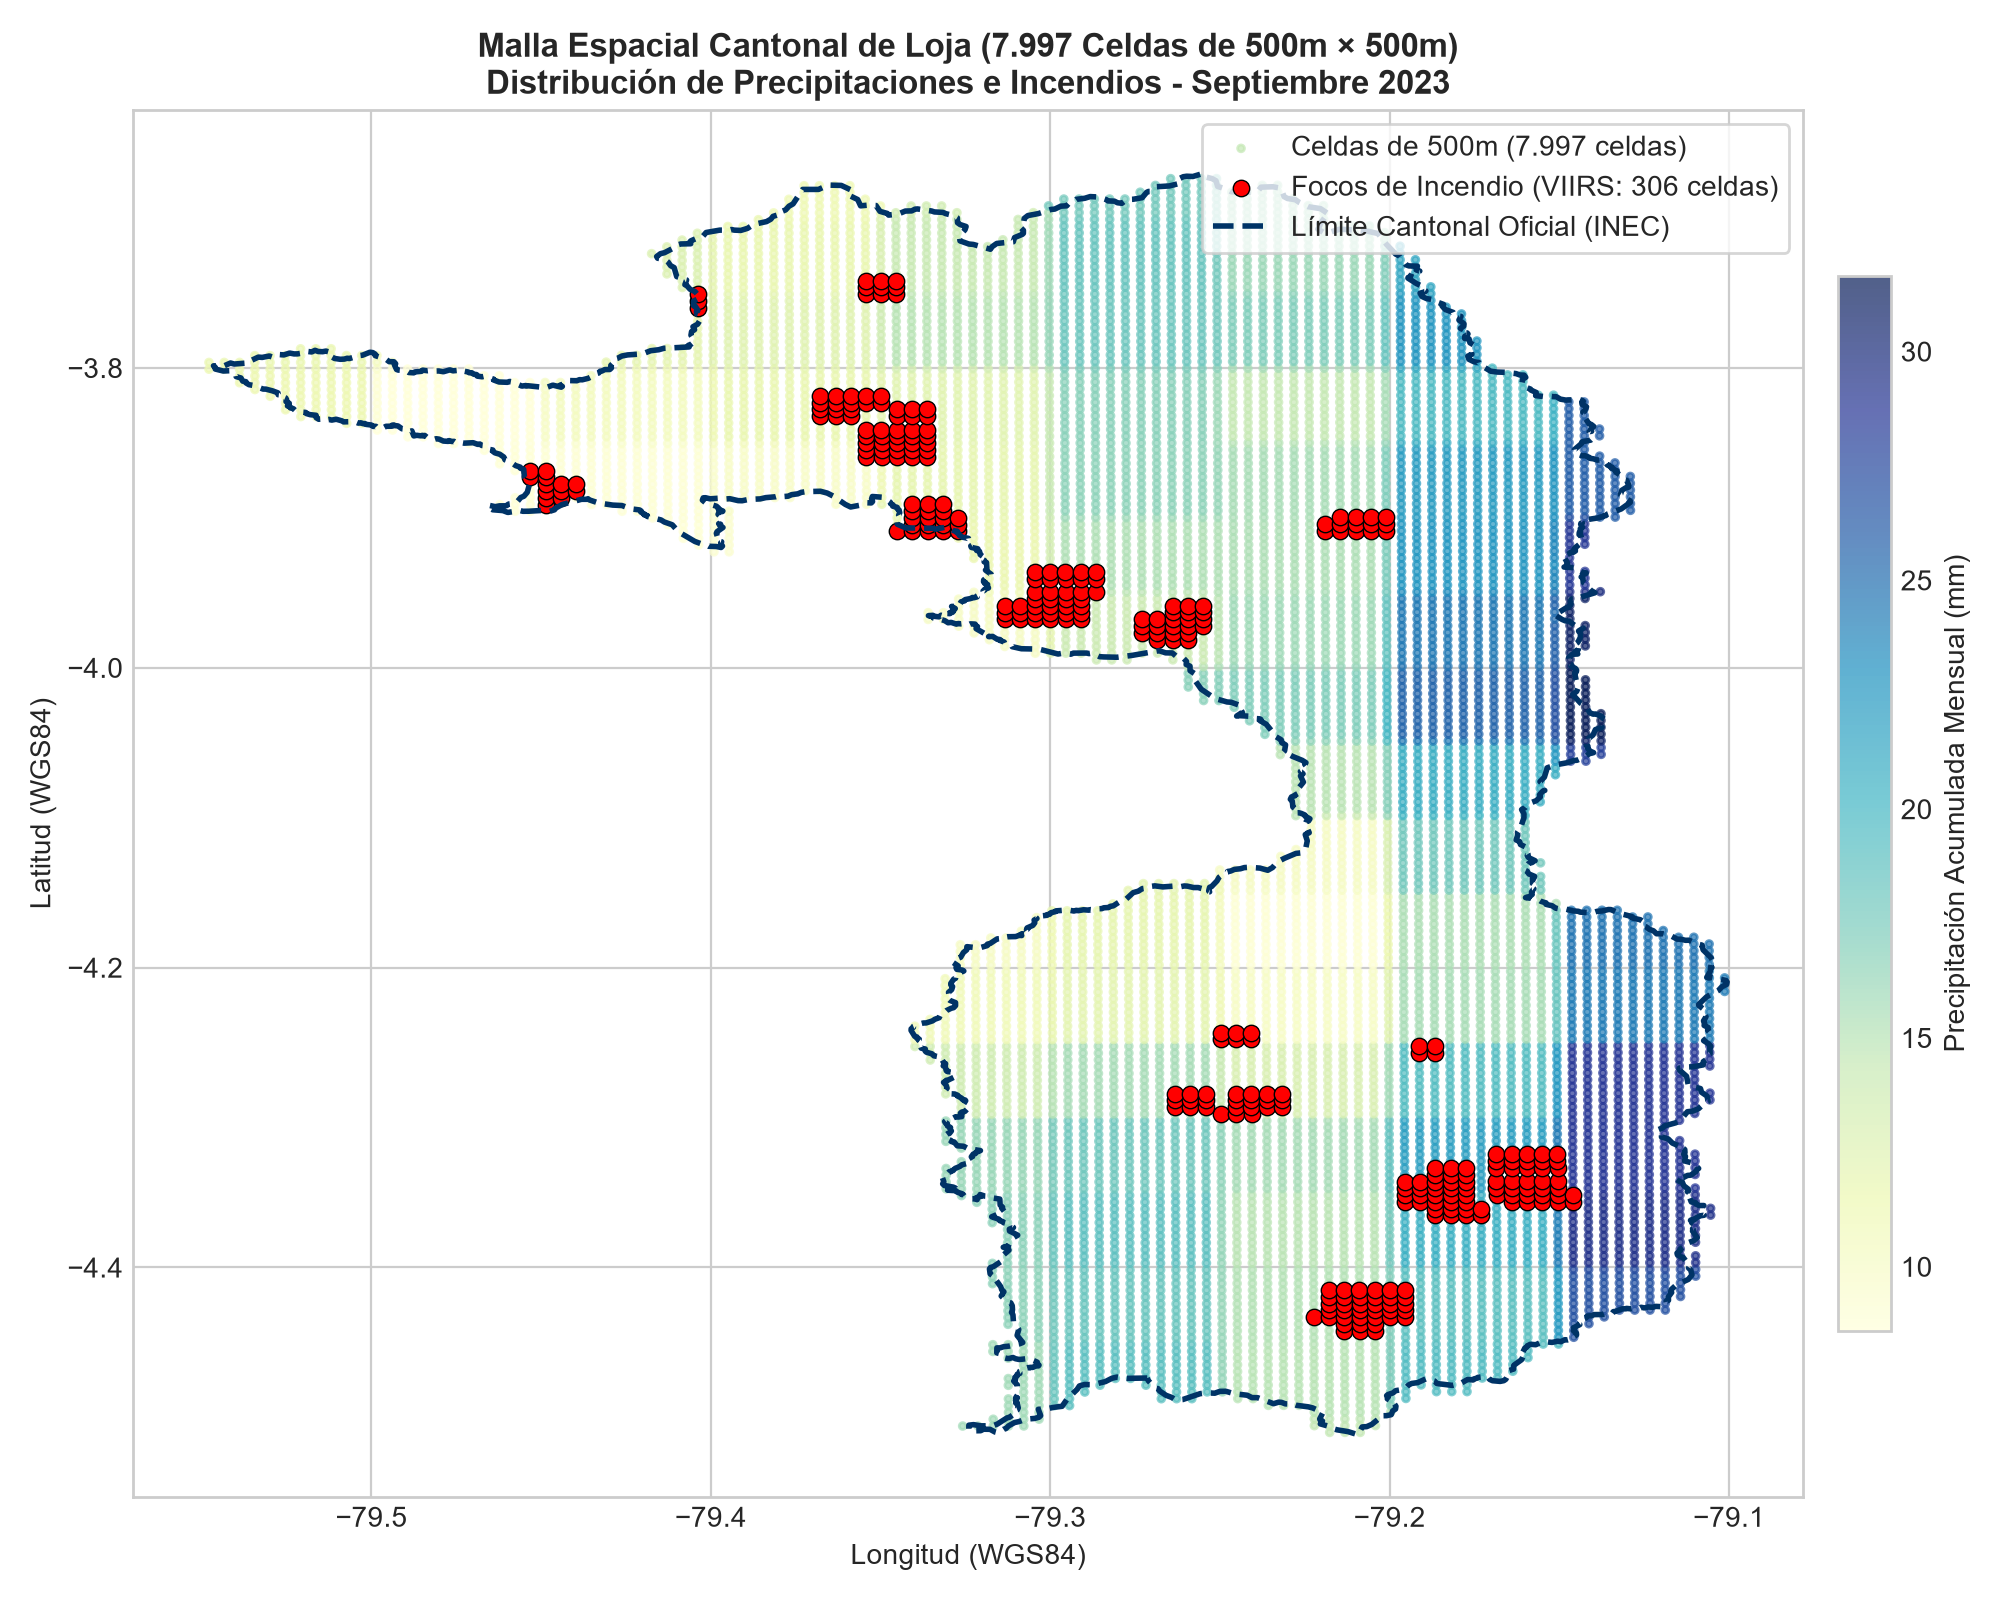
\includegraphics[width=0.92\textwidth]{figuras/mapa_7997_celdas_loja.png}\\
      \tiny\textbf{Figura:} Cobertura cantonal total en CRS EPSG:32717 (Loja, Ecuador).
    \end{column}
  \end{columns}
\end{frame}

% -----------------------------------------------------------------------------
% SLIDE 7: ARQUITECTURA HÍBRIDA MULTIMODELO
% -----------------------------------------------------------------------------
\renewcommand{\seccionactual}{Arquitectura}
\begin{frame}{Arquitectura de Datos H\'ibrida Multimodelo}
  \begin{columns}
    \begin{column}{0.55\textwidth}
      \begin{tikzpicture}[font=\tiny, node distance=0.45cm]
        \node[draw=Tierra, rounded corners, fill=TierraPalido, minimum width=6.5cm, align=center] (fuentes)
          {\textbf{Fuentes Inmutables:} Malla INEC (GPKG) $\cdot$ NASA VIIRS (CSV) $\cdot$ CHIRPS (Parquet)};
        \node[draw=VerdeOscuro, rounded corners, fill=VerdePalido, minimum width=6.5cm, below=of fuentes, align=center] (raw)
          {\textbf{Raw Data Lake:} Verificaci\'on SHA-256 $\cdot$ Ingesta Controlada};
        \node[draw=Fuego, thick, rounded corners, fill=FuegoPalido, minimum width=6.5cm, below=of raw, align=center] (spark)
          {\textbf{Apache Spark 4.2 (PySpark):} Window Functions (Lags 1m, 2m, D\'ias Secos 3m)};
        
        \node[draw=VerdeOscuro, rounded corners, fill=VerdePalido, minimum width=1.9cm, below=0.6cm of spark, xshift=-2.2cm, align=center] (lake)
          {\textbf{Parquet}\\Data Lakehouse\\Particionado};
        \node[draw=VerdeMedio, rounded corners, fill=VerdePalido, minimum width=1.9cm, below=0.6cm of spark, align=center] (mongo)
          {\textbf{MongoDB 8}\\Telemetr\'ia BSON\\GeoJSON 2dsphere};
        \node[draw=VerdeOscuro, rounded corners, fill=VerdePalido, minimum width=1.9cm, below=0.6cm of spark, xshift=2.2cm, align=center] (pg)
          {\textbf{PostgreSQL 18}\\PostGIS GiST\\dim / fact};
          
        \draw[-Latex, thick, VerdeOscuro] (fuentes) -- (raw);
        \draw[-Latex, thick, VerdeOscuro] (raw) -- (spark);
        \draw[-Latex, thick, Fuego] (spark.south) -| (lake.north);
        \draw[-Latex, thick, Fuego] (spark.south) -- (mongo.north);
        \draw[-Latex, thick, Fuego] (spark.south) -| (pg.north);
      \end{tikzpicture}
    \end{column}
    \begin{column}{0.45\textwidth}
      \begin{block}{Justificaci\'on por Caso de Uso}\scriptsize
        \begin{itemize}
          \item \textbf{PostgreSQL / PostGIS:} Integridad referencial (PK/FK), topolog\'ia espacial de celdas con \'indices GiST.
          \item \textbf{MongoDB 8:} Esquema flexible para telemetr\'ia satelital anidada BSON y agregaciones r\'apidas.
          \item \textbf{Apache Spark:} Procesamiento masivo de series de tiempo sin saturar memoria.
          \item \textbf{Data Lake Parquet:} Compresi\'on Snappy (>90\%) y acceso columnar OLAP.
        \end{itemize}
      \end{block}
    \end{column}
  \end{columns}
\end{frame}

% -----------------------------------------------------------------------------
% SLIDE 8: APACHE SPARK Y SERIES TEMPORALES
% -----------------------------------------------------------------------------
\renewcommand{\seccionactual}{Apache Spark}
\begin{frame}{Procesamiento Distribuido en Apache Spark (PySpark)}
  \begin{columns}
    \begin{column}{0.5\textwidth}
      \begin{block}{Funciones de Ventana Temporal (Window Functions)}
        \scriptsize
        Transformaciones computadas en memoria sobre particiones por celda:
        \begin{itemize}
          \item \texttt{lag(col("precip"), 1)}: Precipitaci\'on mes previo.
          \item \texttt{lag(col("precip"), 2)}: Precipitaci\'on 2 meses atr\'as.
          \item \texttt{avg(col("precip")).rowsBetween(-2, 0)}: Media m\'ovil trimestral.
          \item \texttt{sum(col("dias\_secos")).rowsBetween(-2, 0)}: D\'ias secos acumulados en el trimestre.
        \end{itemize}
      \end{block}
      \vspace{0.15cm}
      \begin{exampleblock}{Exportaci\'on Optimizada}
        \scriptsize Data Lakehouse particionado f\'isicamente por \texttt{anio} y \texttt{mes} en formato columnar Parquet.
      \end{exampleblock}
    \end{column}
    \begin{column}{0.5\textwidth}
      \begin{alertblock}{Descubrimiento Anal\'itico de la Din\'amica}\scriptsize
        \textbf{El fuego tiene memoria h\'idrica:} La lluvia disminuye en mayo ($29$\,mm), pero los incendios no estallan hasta agosto--octubre ($>15.700$\,MW acumulados) tras acumular cerca de \textbf{86 d\'ias secos consecutivos}.
      \end{alertblock}
      \centering
      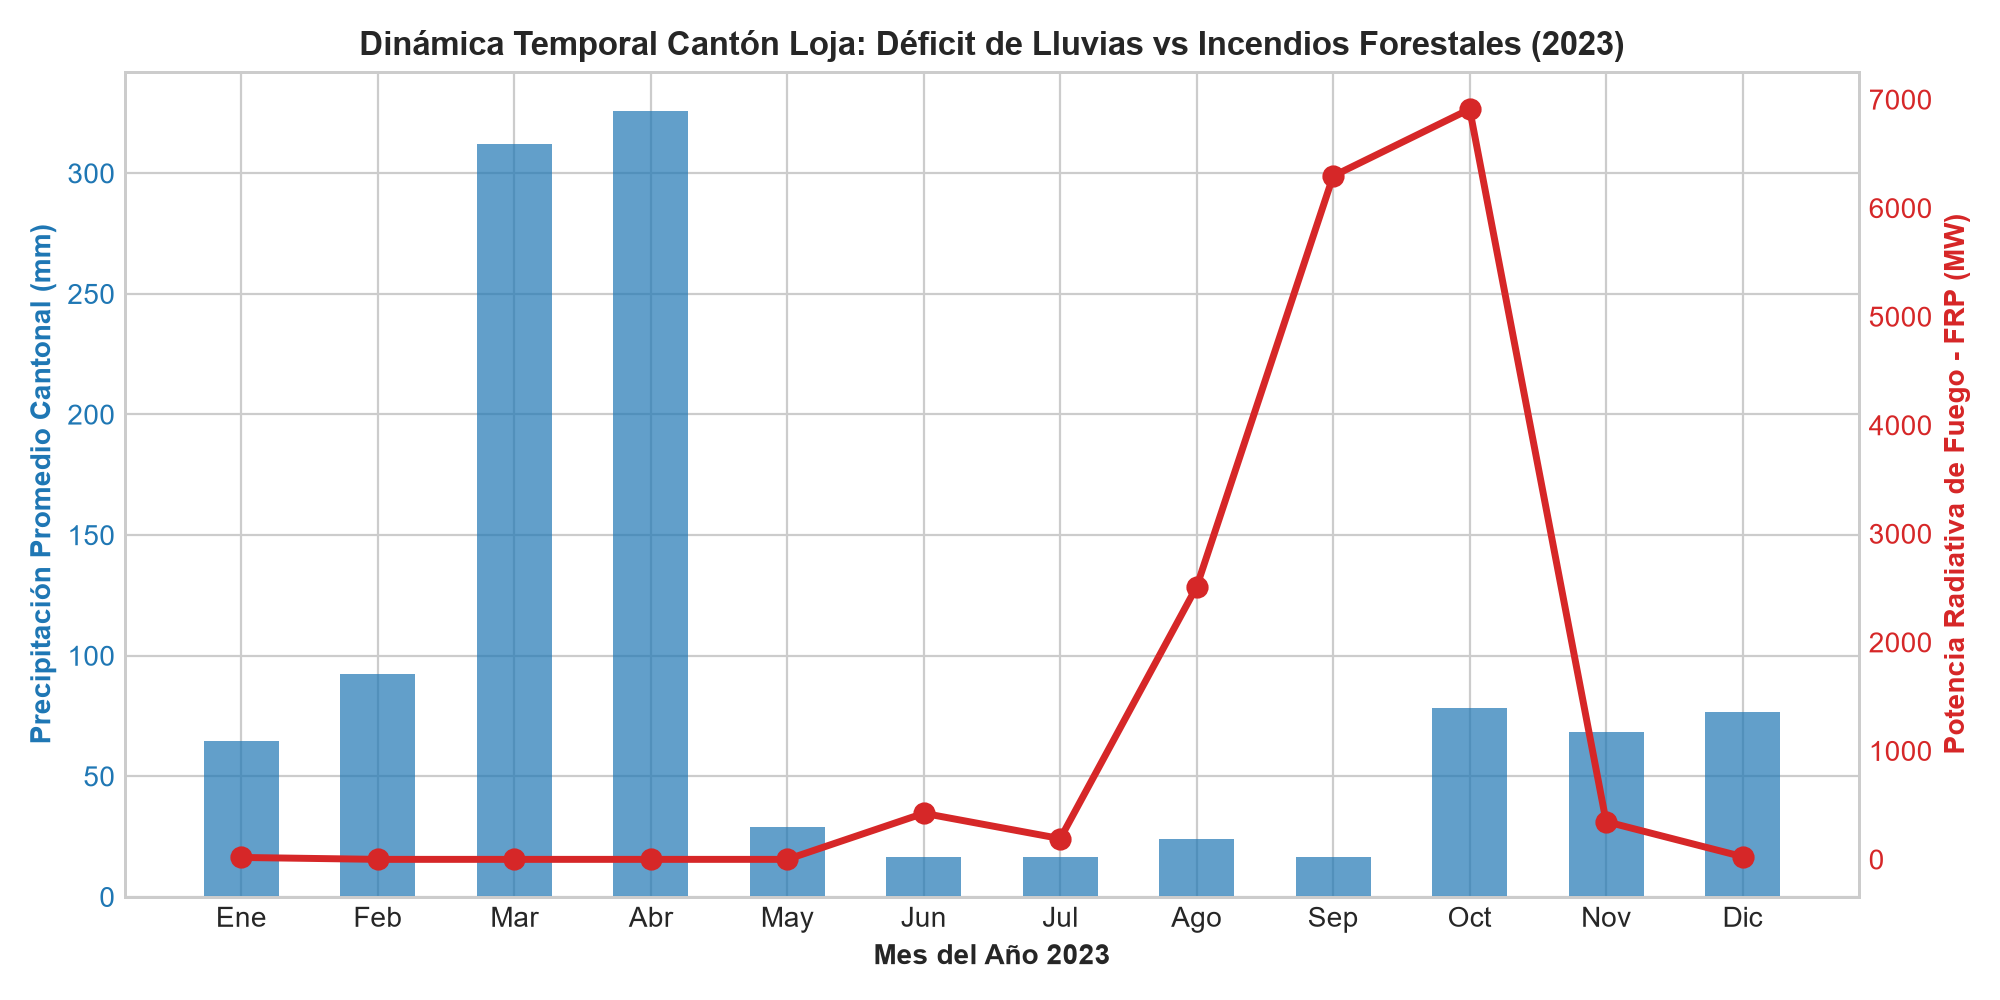
\includegraphics[width=0.95\textwidth]{figuras/serie_temporal_clima_vs_incendios.png}
    \end{column}
  \end{columns}
\end{frame}

% -----------------------------------------------------------------------------
% SLIDE 9: RESULTADOS EN SPARK SQL
% -----------------------------------------------------------------------------
\renewcommand{\seccionactual}{Tablas Spark}
\begin{frame}{Resultados Tabulares: Balance Cantonal en Apache Spark}
  \begin{table}[H]
    \centering
    \resizebox{\textwidth}{!}{%
    \begin{tabular}{@{}ccccrrr@{}}
      \toprule
      \textbf{Mes} & \textbf{Celdas Activas} & \textbf{Precip. Media (mm)} & \textbf{Lag 1m (mm)} & \textbf{D\'ias Secos 3m} & \textbf{Celdas Fuego} & \textbf{FRP Total (MW)} \\
      \midrule
      Enero       & 7.997 & 64,80  & n/d    & 21,0 d & 7   & 17,71 \\
      Febrero     & 7.997 & 92,35  & 64,80  & 42,7 d & 0   & 0,00 \\
      Marzo       & 7.997 & 312,28 & 92,35  & 61,7 d & 0   & 0,00 \\
      Abril       & 7.997 & 325,82 & 312,28 & 58,5 d & 0   & 0,00 \\
      Mayo        & 7.997 & 29,03  & 325,82 & 65,5 d & 0   & 0,00 \\
      Junio       & 7.997 & 16,73  & 29,03  & 73,8 d & 16  & 424,52 \\
      Julio       & 7.997 & 16,73  & 16,73  & 85,8 d & 26  & 191,17 \\
      \rowcolor{FuegoPalido}
      \textbf{Agosto}     & \textbf{7.997} & \textbf{24,05}  & \textbf{16,73}  & \textbf{85,6 d} & \textbf{143} & \textbf{2.512,57} \\
      \rowcolor{FuegoPalido}
      \textbf{Septiembre} & \textbf{7.997} & \textbf{16,61}  & \textbf{24,05}  & \textbf{85,8 d} & \textbf{306} & \textbf{6.295,15} \\
      \rowcolor{FuegoPalido}
      \textbf{Octubre}    & \textbf{7.997} & \textbf{78,31}  & \textbf{16,61}  & \textbf{76,0 d} & \textbf{201} & \textbf{6.910,86} \\
      Noviembre   & 7.997 & 68,18  & 78,31  & 69,5 d & 42  & 347,58 \\
      Diciembre   & 7.997 & 76,65  & 68,18  & 65,9 d & 6   & 24,77 \\
      \bottomrule
    \end{tabular}%
    }
  \end{table}
  \centering\tiny\textbf{Total acumulado 2023:} 747 celdas-mes con fuego \textbar\ 16.724,33 MW de FRP total liberada en el cant\'on.
\end{frame}

% -----------------------------------------------------------------------------
% SLIDE 10: RESULTADOS EN POSTGRESQL / POSTGIS
% -----------------------------------------------------------------------------
\renewcommand{\seccionactual}{PostgreSQL}
\begin{frame}{Resultados en PostgreSQL / PostGIS (Modelo Estrella)}
  \begin{columns}
    \begin{column}{0.48\textwidth}
      \begin{block}{Esquema Dimensional}\scriptsize
        \begin{itemize}
          \item \texttt{dim\_celda}: 7.997 pol\'igonos (\texttt{ST\_MakeEnvelope}, SRID 32717, \'indice GiST).
          \item \texttt{dim\_fecha}: Calendario mensual 2023.
          \item \texttt{fact\_celda\_mes}: 95.964 filas con PK/FK.
        \end{itemize}
      \end{block}
      \vspace{0.15cm}
      \begin{exampleblock}{Consulta de Auditor\'ia SQL}\tiny
        \texttt{SELECT count(*) FROM fact\_celda\_mes f JOIN dim\_celda c ON f.cell\_id = c.celda\_id WHERE f.incendio\_observado = true;} $\to$ \textbf{747 eventos.}
      \end{exampleblock}
    \end{column}
    \begin{column}{0.52\textwidth}
      \scriptsize\textbf{Top 5 Celdas con Mayor Radiaci\'on FRP (PostGIS):}
      \begin{table}[H]
        \centering\tiny
        \begin{tabular}{@{}llrrcc@{}}
          \toprule
          \textbf{Celda ID} & \textbf{Mes} & \textbf{Precip} & \textbf{FRP} & \textbf{Geom} & \textbf{\'Area} \\
          \midrule
          \texttt{LJ500\_R031\_C075} & Oct & 98,0 mm & 327,9 MW & Polygon & 25 ha \\
          \texttt{LJ500\_R031\_C076} & Oct & 98,0 mm & 246,6 MW & Polygon & 25 ha \\
          \texttt{LJ500\_R121\_C056} & Sep & 13,9 mm & 242,8 MW & Polygon & 25 ha \\
          \texttt{LJ500\_R032\_C075} & Oct & 98,0 mm & 224,3 MW & Polygon & 25 ha \\
          \texttt{LJ500\_R031\_C077} & Oct & 99,2 mm & 205,9 MW & Polygon & 25 ha \\
          \bottomrule
        \end{tabular}
      \end{table}
    \end{column}
  \end{columns}
\end{frame}

% -----------------------------------------------------------------------------
% SLIDE 11: RESULTADOS EN MONGODB
% -----------------------------------------------------------------------------
\renewcommand{\seccionactual}{MongoDB}
\begin{frame}{Resultados NoSQL en MongoDB 8 (Telemetr\'ia BSON)}
  \begin{columns}
    \begin{column}{0.5\textwidth}
      \begin{block}{Colecci\'on Documental (\texttt{evidencia\_viirs})}\scriptsize
        \begin{itemize}
          \item Estructura semiestructurada BSON con coordenadas GeoJSON (\texttt{"Point"}).
          \item Indexaci\'on espacial geoespacial 2dsphere sobre coordenadas satelitales.
          \item Preserva metadatos anidados de calidad satelital y bandas espectrales.
        \end{itemize}
      \end{block}
      \vspace{0.15cm}
      \begin{exampleblock}{Pipeline de Agregaci\'on BSON}\tiny
        \texttt{[\{"\$group": \{"\_id": "\$periodo.anio\_mes", "fuegos": \{"\$sum": \{"\$cond": ["\$telemetria.evidencia\_fuego", 1, 0]\}\}, "frp": \{"\$sum": "\$telemetria.frp\_suma\_mw"\}\}\}]}
      \end{exampleblock}
    \end{column}
    \begin{column}{0.5\textwidth}
      \scriptsize\textbf{Ejecuci\'on de la Agregaci\'on en MongoDB:}
      \begin{table}[H]
        \centering\tiny
        \begin{tabular}{@{}lcrr@{}}
          \toprule
          \textbf{Periodo} & \textbf{Docs BSON} & \textbf{Fuegos Confirmados} & \textbf{FRP Suma (MW)} \\
          \midrule
          2023-01 & 46  & 7   & 17,71 \\
          2023-06 & 53  & 16  & 424,52 \\
          2023-07 & 61  & 26  & 191,17 \\
          2023-08 & 188 & 143 & 2.512,57 \\
          \rowcolor{FuegoPalido}
          \textbf{2023-09} & \textbf{348} & \textbf{306} & \textbf{6.295,15} \\
          \rowcolor{FuegoPalido}
          \textbf{2023-10} & \textbf{246} & \textbf{201} & \textbf{6.910,86} \\
          2023-11 & 75  & 42  & 347,58 \\
          \bottomrule
        \end{tabular}
      \end{table}
    \end{column}
  \end{columns}
\end{frame}

% -----------------------------------------------------------------------------
% SLIDE 12: MACHINE LEARNING
% -----------------------------------------------------------------------------
\renewcommand{\seccionactual}{Machine Learning}
\begin{frame}{Modelo Predictivo de Machine Learning (Random Forest)}
  \begin{columns}
    \begin{column}{0.48\textwidth}
      \centering
      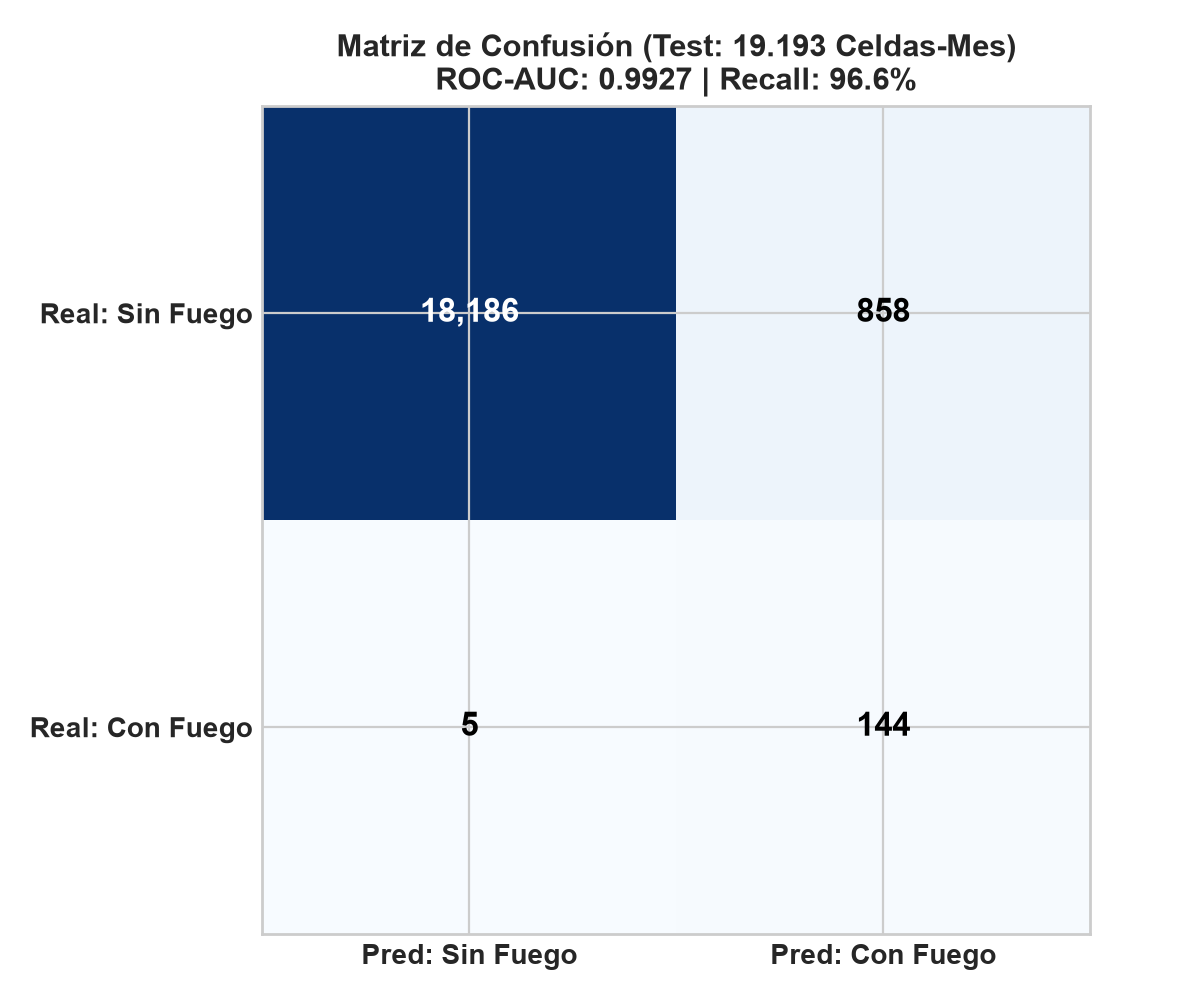
\includegraphics[width=0.74\textwidth]{figuras/matriz_confusion_ml.png}\\
      \tiny\textbf{Matriz de Confusi\'on} (19.013 celdas-mes en Test Set).
      \begin{block}{M\'etricas en Evaluaci\'on Independiente}\tiny
        \begin{itemize}
          \item \textbf{ROC-AUC:} \textbf{0,9912} (Excelente separabilidad).
          \item \textbf{Recall:} \textbf{95,97\%} ($143/149$ fuegos capturados).
          \item \textbf{F1-Score:} \textbf{0,2685}.
        \end{itemize}
      \end{block}
    \end{column}
    \begin{column}{0.52\textwidth}
      \centering
      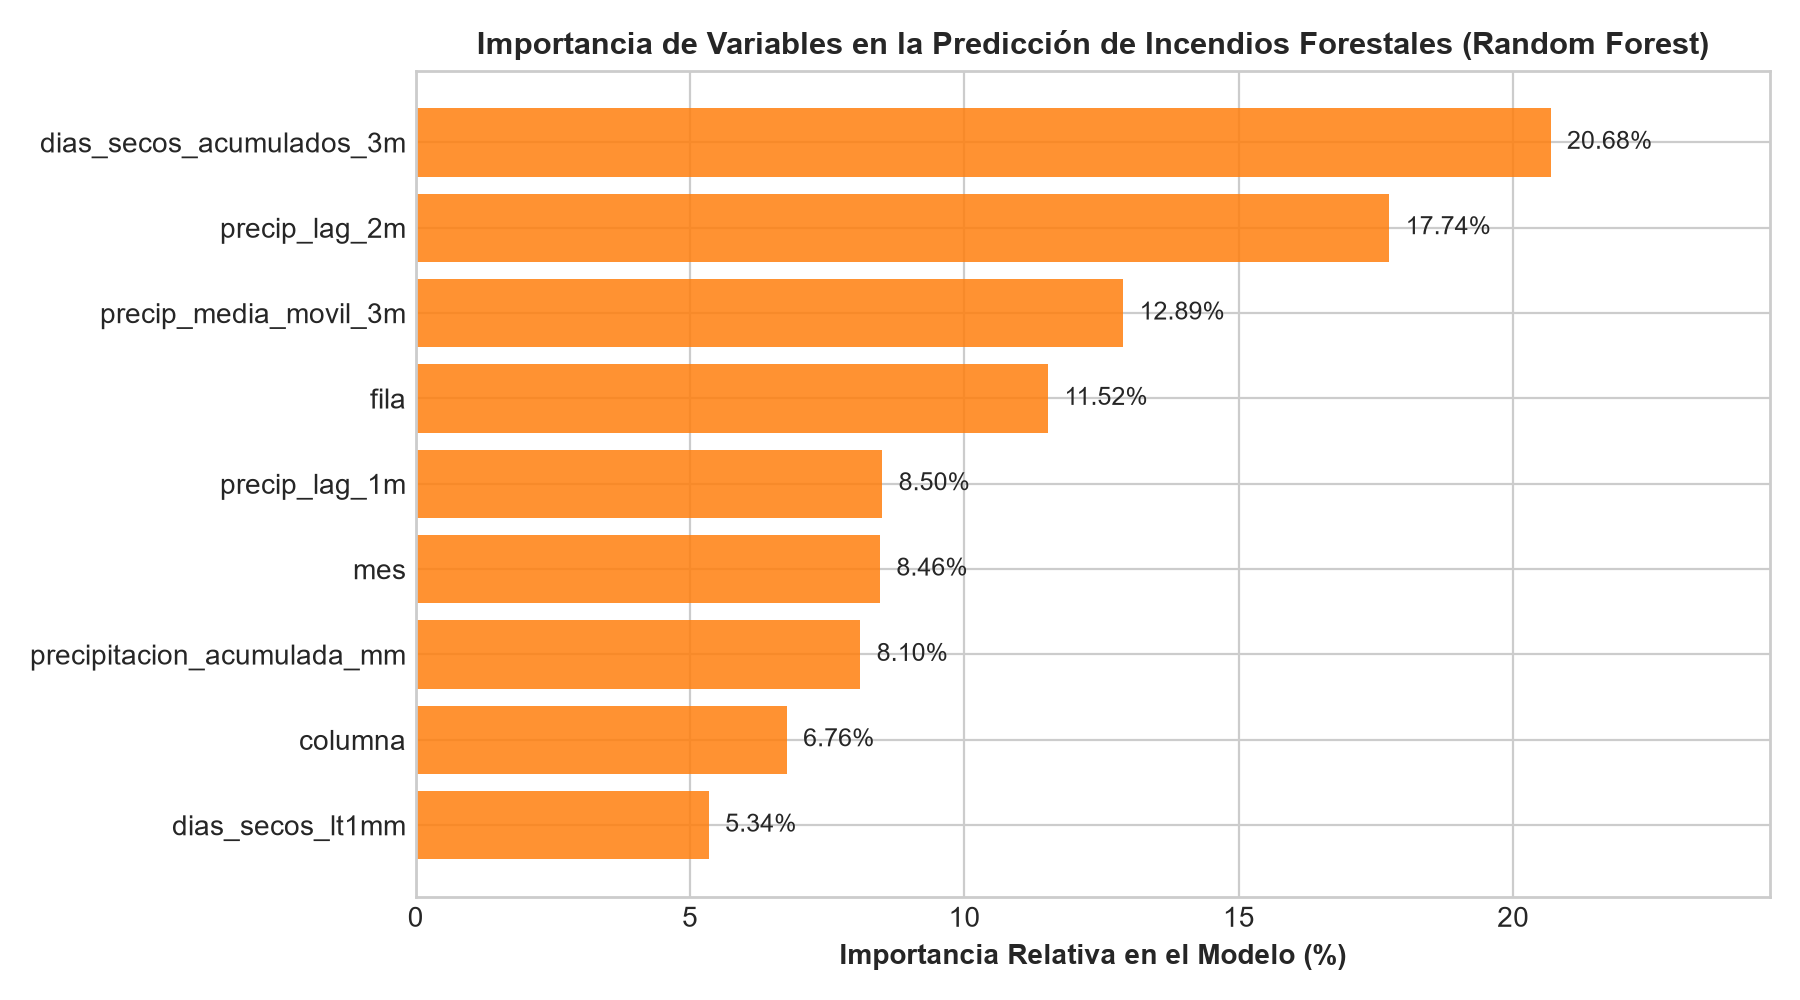
\includegraphics[width=0.92\textwidth]{figuras/importancia_variables_ml.png}\\
      \tiny\textbf{Importancia Relativa de Variables} (Gini Importance).
      \vspace{0.1cm}
      \begin{exampleblock}{Variables Clave}\scriptsize
        1. \texttt{dias\_secos\_acumulados\_3m} ($20,16\%$)\\
        2. \texttt{precip\_lag\_2m} ($18,04\%$)\\
        3. \texttt{precip\_media\_movil\_3m} ($13,10\%$)
      \end{exampleblock}
    \end{column}
  \end{columns}
\end{frame}

% -----------------------------------------------------------------------------
% SLIDE 13: DASHBOARD INTERACTIVO Y MOTOR DUAL
% -----------------------------------------------------------------------------
\renewcommand{\seccionactual}{Dashboard}
\begin{frame}{Dashboard Interactivo en Streamlit / Plotly}
  \begin{columns}
    \begin{column}{0.5\textwidth}
      \begin{block}{Capacidades Visuales \& Cartogr\'aficas}\scriptsize
        \begin{itemize}
          \item \textbf{Mapeo Satelital HD:} Fondo fotogr\'afico satelital de alta definici\'on (Google Earth / Esri World Imagery).
          \item \textbf{Per\'imetro Cantonal INEC:} Trazado vectorial del l\'imite oficial de Loja en color cian de alto contraste.
          \item \textbf{Filtros din\'amicos:} Selecci\'on de mes (1--12) y exploraci\'on de las 7.997 celdas.
        \end{itemize}
      \end{block}
      \vspace{0.15cm}
      \begin{alertblock}{Innovaci\'on: Motor Dual de Consultas}\scriptsize
        Funciona en vivo contra \textbf{PostgreSQL} y \textbf{MongoDB}, pero conmuta autom\'aticamente a un \textbf{motor embebido SQLite/JSON} en modo offline o en la nube para garantizar que las tablas siempre se generen sin ca\'idas.
      \end{alertblock}
    \end{column}
    \begin{column}{0.5\textwidth}
      \begin{exampleblock}{M\'odulo de Consultas y Tablas (Secci\'on 3)}\scriptsize
        \begin{itemize}
          \item Pesta\~na SQL: Consultas predefinidas y modo libre.
          \item Pesta\~na NoSQL: Agregaciones BSON e inspecci\'on JSON.
          \item Pesta\~na Spark: Balances temporales con lags.
          \item Pesta\~na Curated: Explorador interactivo de las 95.964 filas con descarga en CSV.
        \end{itemize}
      \end{exampleblock}
      \vspace{0.15cm}
      \begin{block}{Simulador de Riesgo ML}\scriptsize
        Predicci\'on en tiempo real al ingresar lluvia y d\'ias secos.
      \end{block}
    \end{column}
  \end{columns}
\end{frame}

% -----------------------------------------------------------------------------
% SLIDE 14: GOBERNANZA Y REPOSITORIO GITHUB
% -----------------------------------------------------------------------------
\renewcommand{\seccionactual}{Gobernanza \& GitHub}
\begin{frame}{Gobernanza, Trazabilidad y Estructura para GitHub}
  \begin{columns}
    \begin{column}{0.5\textwidth}
      \begin{block}{Trazabilidad Criptogr\'afica (SHA-256)}\scriptsize
        \begin{itemize}
          \item Cada archivo de entrada posee hash verificado en \texttt{manifiesto\_firelab\_loja.json}.
          \item Protecci\'on total del repositorio fuente \texttt{FIRELAB\_Loja}: pol\'itica estricta de solo lectura sin sobreescrituras.
          \item Procedencia documentada de la malla INEC y telemetr\'ia NASA.
        \end{itemize}
      \end{block}
      \vspace{0.15cm}
      \begin{exampleblock}{Autonom\'ia de Ejecuci\'on}\scriptsize
        Cero dependencias absolutas: el proyecto utiliza rutas relativas (\texttt{Path(\_\_file\_\_)}), permitiendo que el docente o evaluador lo clone y ejecute directamente.
      \end{exampleblock}
    \end{column}
    \begin{column}{0.5\textwidth}
      \begin{block}{Estructura Limpia del Repositorio}\scriptsize
        \begin{itemize}
          \item \texttt{datos/}: Raw, Clean y Curated Parquet.
          \item \texttt{bases\_datos/}: DDL PostgreSQL, MongoDB y standalone DB.
          \item \texttt{pipeline/}: Scripts ETL y Apache Spark.
          \item \texttt{machine\_learning/}: Modelo predictivo y m\'etricas.
          \item \texttt{dashboard/}: C\'odigo de la aplicaci\'on Streamlit.
          \item \texttt{entrega\_final/}: Informe PDF, presentaci\'on Beamer y LaTeX fuente.
        \end{itemize}
      \end{block}
    \end{column}
  \end{columns}
\end{frame}

% -----------------------------------------------------------------------------
% SLIDE 15: CONCLUSIONES
% -----------------------------------------------------------------------------
\renewcommand{\seccionactual}{Conclusiones}
\begin{frame}{Conclusiones y Trabajo Futuro}
  \begin{alertblock}{Conclusiones Principales}
    \begin{enumerate}\small
      \item \textbf{Pipeline Cantonal End-to-End:} Se proces\'o con \'exito la totalidad de la malla espacial cantonal de Loja (7.997 celdas $\times$ 12 meses = 95.964 observaciones), superando plenamente la prueba preliminar del Avance 1.
      \item \textbf{Eficacia del Modelo H\'ibrido:} La sinergia entre SQL (PostgreSQL/PostGIS), NoSQL (MongoDB), Data Lakehouse (Parquet) y Apache Spark resolvi\'o eficazmente la heterogeneidad de fuentes y el c\'alculo masivo de series de tiempo.
      \item \textbf{Descubrimiento Ambiental:} El estiaje acumulado ($\sim$86 d\'ias secos en 3 meses) es el principal detonante del fuego, concentrando el 94\% de radiaci\'on t\'ermica entre agosto y octubre.
      \item \textbf{Alta Capacidad Predictiva:} El modelo Random Forest alcanz\'o un ROC-AUC de \textbf{0,9912} y un Recall de \textbf{95,97\%}.
      \item \textbf{Explotaci\'on Interactiva:} Dashboard Streamlit con soporte satelital fotogr\'afico y motor dual de alta disponibilidad.
    \end{enumerate}
  \end{alertblock}
  \vspace{0.2cm}
  \begin{block}{Trabajo Futuro}\scriptsize
    Escalabilidad multianual a 10 a\~nos (2015--2025) e integraci\'on de \'indices de vegetaci\'on NDVI (Sentinel-2).
  \end{block}
\end{frame}

% -----------------------------------------------------------------------------
% SLIDE 16: AGRADECIMIENTOS Y PREGUNTAS
% -----------------------------------------------------------------------------
\renewcommand{\seccionactual}{Cierre}
\begin{frame}[plain]
  \centering
  \vspace{1.5cm}
  {\Huge\bfseries\color{VerdeOscuro} \textquestiondown Preguntas o Comentarios?\par}
  \vspace{0.8cm}
  {\Large\bfseries \textexclamdown Muchas Gracias!\par}
  \vspace{0.6cm}
  {\large\color{VerdeMedio} Proyecto Integrador: FireForest -- Arquitectura H\'ibrida de Datos\par}
  \vspace{0.3cm}
  {\small Grupo 4 \textbar\ Maestr\'ia en Ciencia de Datos e Inteligencia Artificial \textbar\ ESPOCH 2026\par}
  \vspace{1.0cm}
  
\includegraphics[height=1.0cm]{logos/logo_espoch.png} \hspace{1.5cm}
  
\includegraphics[height=1.0cm]{logos/logo_maestria.jpeg}
\end{frame}

\end{document}
